\newpage
\section{Isomorphism Theorems}

\begin{theorem}[First Isomorphism Theorem] \label{thm:iso1}
    If $\varphi \colon G \to H$ is a group homomorphism, then $G/\ker\varphi \cong \im\varphi$.
\end{theorem}
\begin{proof}
    Let $N$ be $\ker\varphi$ and let $G^{\prime} = \im\varphi$. We have shown that $N \trianglelefteq G$. Let $\pi \colon G \to G/N$ be the map defined as $\pi(g) = gN$ for all $g \in G$. Now, we define $\psi \colon G/N \to G^{\prime}$ as $\psi(gN) = \varphi(g)$ for all $gN \in G/N$. We first show that this map is well-defined. For $g,h \in G$, we have
    \[
        gN = hN \iff h^{-1}g \in N \iff \varphi(h^{-1}g) = 1 \iff (\varphi(h))^{-1} \varphi(g) = 1 \iff \varphi(g) = \varphi(h)
    \]
    This not only proves that the map is well-defined but also that it is injective. Moreover, surjectivity of $\psi$ is easy to verify. Hence, $\psi$ is an isomorphism between $G/N$ and $G^{\prime}$. Recall that we had defined $N = \ker\varphi$ and $G^{\prime} = \im\varphi$. Thus, $G/\ker\varphi \cong \im\varphi$.
\end{proof}

Pictorially, we can visualise the first isomorphism theorem as follows.

\begin{center}
\begin{tikzpicture}[->, >=stealth', node distance=2cm]
    \node (G) {$G$};
    \node[right of=G] (H) {$\im\varphi$};
    \node[below of=H] (GN) {$G/\ker\varphi$};
    \draw (G) edge[above] node {$\varphi$} (H)
          (GN) edge[right] node {$\psi$} (H)
          (G) edge[below left] node {$\pi$} (GN);
\end{tikzpicture}
\end{center}

For example, consider $\varphi \colon S_n \to \{1,-1\}$ defined by $\varphi(\sigma) = \sign\sigma$ for all $\sigma \in S_n$. The kernel of this map is the group of all even permutations, or the alternating group. Thus, $\ker\varphi = A_n$. By the first isomorphism theorem, $S_n/A_n \cong \{1,-1\}$ Note that $\{1,-1\}$ is just the cyclic group of order $2$, denoted as $C_2$. Hence, $S_n/A_n \cong C_2$.

\medskip

Let $V$ be the Klein-four group in $S_4$, that is, $V = \left\{ 1, (1\, 2)(3\, 4), (1\, 3)(2\, 4), (1\, 4)(2\, 3) \right\}$. We have seen that $V \trianglelefteq S_4$. After a laborious argument earlier, we were able to show that $S_4/V$ was in fact $S_3$. But this is achieved rather simply using the first isomorphism theorem. We leave it as an exercise to show that $S_4/V \cong S_3$.

\medskip

Let $S^1 \leq \C^{\times}$ be the subgroup of complex numbers with magnitude unity. We define a map $f \colon \R \to S^1$ defined as $f(x) = e^{2\pi ix}$. We leave it as an exercise to show that $f$ is a homomorphism. Notice that $\ker f = \Z$. This shows us that $\Z \trianglelefteq \R$. Moreover, $\R/\Z \cong S^1$.

\begin{theorem}[Second Isomorphism Theorem] \label{thm:iso2}
    Let $G$ be a group. Let $N \trianglelefteq G$ and $H \leq G$. Then, $N \trianglelefteq HN$, $H\cap N \trianglelefteq H$ and $HN/N \cong H/H\cap N$.
\end{theorem}
\begin{proof}
    Since $N$ forms a normal subgroup of $G$, it is also clear that it forms a normal subgroup $HN$. Let $\pi \colon G \to G/N$ be the `natural' homomorphism, that is, $\pi(g) = gN$ for all $g \in G$. Using $\pi$, we define $\pi_H \colon H \to G/N$ which is the restriction of $\pi$ to $H$. It is easy to verify that this restriction is a homomorphism too. We will now show that $\im\pi_H$ is precisely $HN/N$. We have
    \[
        HN/N = \left\{ hnN \mid h \in H, n \in N \right\} = \left\{ (hN)(nN) \mid h \in H, n \in N \right\} = \left\{ hN \mid h \in H \right\} = \im\pi_H
    \]
    Also, $h \in \ker\pi_H \iff hN = N \iff h \in N$. But, we already know that $h \in H$. Hence, $\ker\pi_H$ is given precisely by $H \cap N$. This shows us that $H \cap N \trianglelefteq H$ since it is the kernel of some group homomorphism. By the \nameref{thm:iso1}, we have $H/\ker\pi_H \cong \im\pi_H$ and thus $HN/N \cong H/H\cap N$.
\end{proof}

The second isomorphism theorem is sometimes also called the \emph{Diamond Isomorphism Theorem}, the reason for which should be clear from the following diagram.

\begin{center}
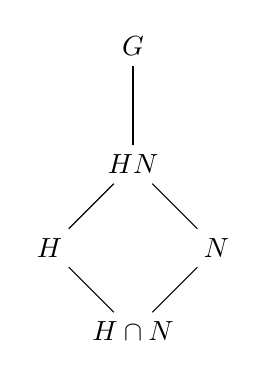
\begin{tikzpicture}[node distance=1.5cm]
    \node (G) {$G$};
    \node[below of=G] (HN) {$HN$};
    \node[below right of=HN] (N) {$N$};
    \node[below left of=HN] (H) {$H$};
    \node[below right of=H] (HiN) {$H\cap N$};
    \draw (G) edge (HN)
          (HN) edge (H)
          (HN) edge[above right] node {$\trianglelefteq$} (N)
          (H) edge[below left] node {$\trianglelefteq$} (HiN)
          (N) edge (HiN);
\end{tikzpicture}
\end{center}

\begin{theorem}[Third Isomorphism Theorem] \label{thm:iso3}
    Let $G$ be a group and let $H,N$ be normal subgroups of $G$ such that $N \leq H$. Then, $(H/N) \trianglelefteq (G/N)$ and $G/H \cong \ddfrac{G/N}{H/N}$.
\end{theorem}
\begin{center}
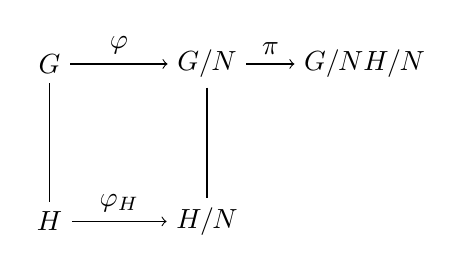
\begin{tikzpicture}[node distance=2cm]
    \node (G) {$G$};
    \node[below of=G] (H) {$H$};
    \node[right of=G] (G/N) {$G/N$};
    \node[below of=G/N] (H/N) {$H/N$};
    \node[right of=G/N] (GNHN) {$\ddfrac{G/N}{H/N}$};
    \draw   (G) edge[left] node {$\trianglelefteq$} (H)
            (G/N) edge[right] node {$\trianglelefteq$} (H/N);
    \path[->]
        (G) edge[above] node {$\varphi$} (G/N)
        (H) edge[above] node {$\varphi_H$} (H/N)
        (G/N) edge [above] node {$\pi$} (GNHN);
\end{tikzpicture}
\end{center}
\begin{proof}
    We will use the above diagrammatic representation to prove this theorem. $\varphi \colon G \to G/N$ represents the natural homomorphism $\varphi(g) = gN$. $\varphi_H$ is the restriction of $\varphi$ to $H$. Let $X \in H/N$ and $Y \in G/N$. We have $X = hN$ for some $h \in H$ and $Y = gN$ for some $g \in G$. Now,
    \[
        YXY^{-1} = (gN)(hN)(g^{-1}N) = (ghg^{-1})N
    \]
    Since $H \trianglelefteq G$, we have that $ghg^{-1} = h^{\prime}$ for some $h^{\prime} \in H$. Thus, $YXY^{-1} = h^{\prime} N \in H/N$ and hence, $H/N \trianglelefteq G/N$. Consider the map $\pi \circ \varphi \colon G \to \ddfrac{G/N}{H/N}$. Since $\pi$ and $\varphi$ are surjective homomorphisms, $\pi \circ \varphi$ is also a surjective homomorphism. We know that $\ker\pi = H/N$. Thus, $\ker(\pi\circ\varphi) = \left\{ g \in G \mid \varphi(g) = H/N \right\}$. Thus, $\ker(\pi\circ\varphi) = H$. By the \nameref{thm:iso1}, we conclude that
    \[
        G/H \cong \frac{G/N}{H/N} \qedhere
    \]
\end{proof}


\begin{theorem} \label{thm:abelian-subgroup-of-order-divisor}
    Let $G$ be a finite abelian group of order $n$ and let $d \in \N^+$ be such that $d \divides n$. Then, $G$ has a subgroup of order $d$.
\end{theorem}
\begin{proof}
    We will apply induction on the order of $G$. If $n = 1$, the theorem is true. Suppose the theorem is true for all abelian groups of order strictly less than $n$. We first prove that for any prime $p$ with $p \divides n$, $G$ has an element of order $p$.
    
    \medskip
    
    We may assume $\abs{G} > 1$. Suppose $a \in G$ such that $\abs{a} = m \geq 2$. Suppose $p \divides m$. Then, $a^{m/p}$ has order $p$. Suppose $p \notdivides m$. Consider $N = \langle a \rangle$ with $\abs{N} = m$. Since $G$ is abelian, every subgroup of $G$ is normal. Hence, $N \trianglelefteq G$. Now, consider the quotient group $G/N$. We know that $\abs{G/N} = n/m$. Since $p \divides n$ and $p \notdivides m$, we conclude that $p$ divides $\abs{G/N}$. By the induction hypothesis, there exists an element of order $p$ in $G/N$, since $G/N$ is abelian and of order strictly less than $n$. Thus, $\abs{bN} = p$ for some $b \in G$. Suppose $\abs{b} = k$. This gives us $b^k = 1 \implies (bN)^k = N$. Thus, $p \divides k$ and we are back to the first case. Hence, there is an element of order $p$ and hence a subgroup of order $p$.
    
    \medskip
    
    Fix a prime $p$ such that $p \divides d$. Let $a \in G$ be an element of order $p$ in $G$ and let $N = \langle a \rangle$. Thus, $\abs{N} = p$. We have $\abs{G/N} = n/p < n$. Now, by the induction hypothesis, there exists a subgroup $H/N$ of $G/N$ with $\abs{H/N} = d/p$. Thus, $\abs{H}/\abs{N} = d/p$, which gives us $\abs{H} = d$ and we are done.
\end{proof}